% Options for packages loaded elsewhere
\PassOptionsToPackage{unicode}{hyperref}
\PassOptionsToPackage{hyphens}{url}
%
\documentclass[
]{article}
\usepackage{lmodern}
\usepackage{amssymb,amsmath}
\usepackage{ifxetex,ifluatex}
\ifnum 0\ifxetex 1\fi\ifluatex 1\fi=0 % if pdftex
  \usepackage[T1]{fontenc}
  \usepackage[utf8]{inputenc}
  \usepackage{textcomp} % provide euro and other symbols
\else % if luatex or xetex
  \usepackage{unicode-math}
  \defaultfontfeatures{Scale=MatchLowercase}
  \defaultfontfeatures[\rmfamily]{Ligatures=TeX,Scale=1}
\fi
% Use upquote if available, for straight quotes in verbatim environments
\IfFileExists{upquote.sty}{\usepackage{upquote}}{}
\IfFileExists{microtype.sty}{% use microtype if available
  \usepackage[]{microtype}
  \UseMicrotypeSet[protrusion]{basicmath} % disable protrusion for tt fonts
}{}
\makeatletter
\@ifundefined{KOMAClassName}{% if non-KOMA class
  \IfFileExists{parskip.sty}{%
    \usepackage{parskip}
  }{% else
    \setlength{\parindent}{0pt}
    \setlength{\parskip}{6pt plus 2pt minus 1pt}}
}{% if KOMA class
  \KOMAoptions{parskip=half}}
\makeatother
\usepackage{xcolor}
\IfFileExists{xurl.sty}{\usepackage{xurl}}{} % add URL line breaks if available
\IfFileExists{bookmark.sty}{\usepackage{bookmark}}{\usepackage{hyperref}}
\hypersetup{
  hidelinks,
  pdfcreator={LaTeX via pandoc}}
\urlstyle{same} % disable monospaced font for URLs
\usepackage{graphicx,grffile}
\makeatletter
\def\maxwidth{\ifdim\Gin@nat@width>\linewidth\linewidth\else\Gin@nat@width\fi}
\def\maxheight{\ifdim\Gin@nat@height>\textheight\textheight\else\Gin@nat@height\fi}
\makeatother
% Scale images if necessary, so that they will not overflow the page
% margins by default, and it is still possible to overwrite the defaults
% using explicit options in \includegraphics[width, height, ...]{}
\setkeys{Gin}{width=\maxwidth,height=\maxheight,keepaspectratio}
% Set default figure placement to htbp
\makeatletter
\def\fps@figure{htbp}
\makeatother
\setlength{\emergencystretch}{3em} % prevent overfull lines
\providecommand{\tightlist}{%
  \setlength{\itemsep}{0pt}\setlength{\parskip}{0pt}}
\setcounter{secnumdepth}{-\maxdimen} % remove section numbering

\date{}

\begin{document}

\hypertarget{header-n0}{%
\section{Nov 19 Tue}\label{header-n0}}

Register Allocation 好難。

\hypertarget{header-n3}{%
\subsubsection{Example}\label{header-n3}}

用上節課最後的例子來看;是 K = 3(三個可用寄存器)的情形。

這裏,給出一個例子。

\hypertarget{header-n6}{%
\paragraph{Registers}\label{header-n6}}

\begin{figure}
\centering

\includegraphics{/Users/yue/Documents/GitHub/2019-2020-autumn-semester/11-november/19.assets/image-20191119080224800.png}
\caption{}
\end{figure}

R1:Return Value 所在的寄存器。

R2:Caller Saved。由調用者負責保存。

R3:Callee Saved。由被調用者負責保存。

\hypertarget{header-n11}{%
\paragraph{Spilling Criteria}\label{header-n11}}

我們用了一個相對客觀的方法來決定 Spill 誰。

udol = Usage and Definition Outside Loop

udil = Usage and Definition Inside Loop

d = Node's Degree

Spill Priority = \(\frac {(udol + 10\times udil)} d\)

Priority 越低,Spilling 優先級別越高。

\hypertarget{header-n18}{%
\paragraph{Coalesce}\label{header-n18}}

我們在做 Coalesce 的時候,例如在這裡,希望將 b 同 r2 做
Coalesce,此時需要逐個檢視他的鄰居們。

鄰居 d 的 Degree = 2(數度不數虛線),小於
3,因此完全無需納入考慮。他不是個問題。

\begin{figure}
\centering
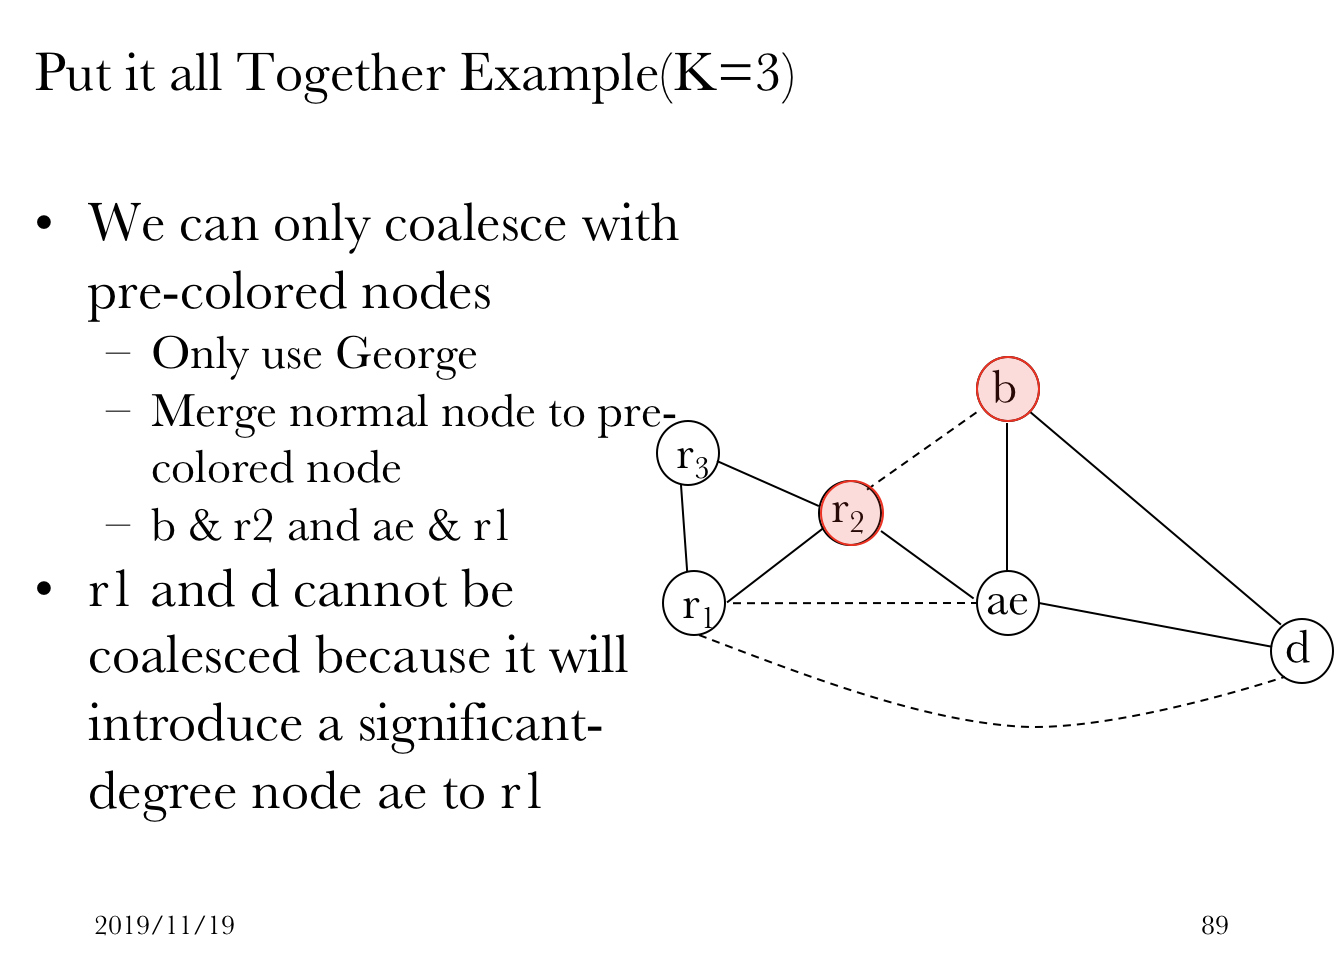
\includegraphics{/Users/yue/Documents/GitHub/2019-2020-autumn-semester/11-november/19.assets/image-20191119081919378.png}
\caption{}
\end{figure}

而對 d 同 r1,就無法做 Coalesce,因為這樣 ae 到 r1 間有 Hard
Link(硬實線)。

\begin{figure}
\centering
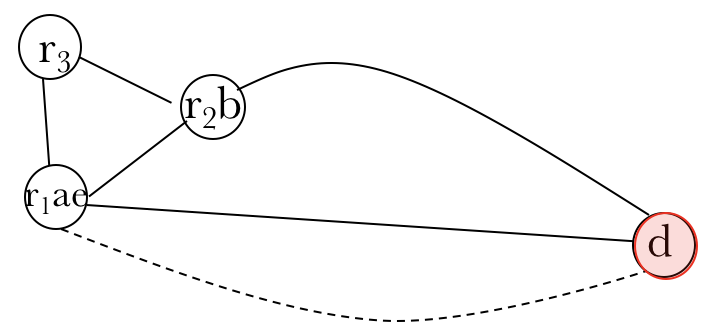
\includegraphics{/Users/yue/Documents/GitHub/2019-2020-autumn-semester/11-november/19.assets/image-20191119082456924.png}
\caption{}
\end{figure}

\hypertarget{header-n25}{%
\paragraph{Finally}\label{header-n25}}

\begin{figure}
\centering
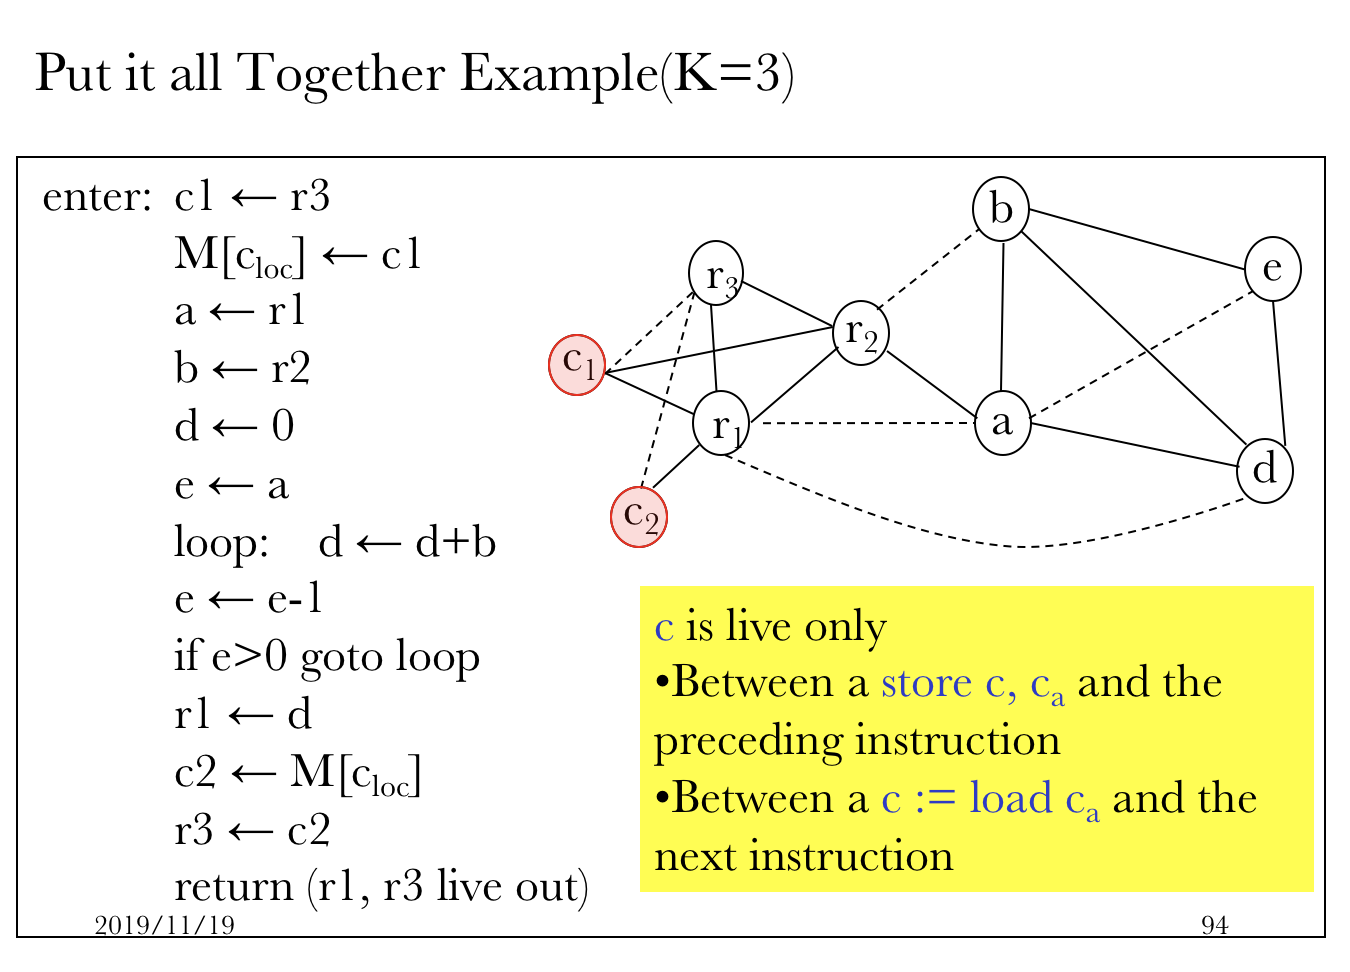
\includegraphics{/Users/yue/Documents/GitHub/2019-2020-autumn-semester/11-november/19.assets/image-20191119082721503.png}
\caption{}
\end{figure}

最後我們得到的結果就是這樣。

留意我們用了 Callee Saved Register R3。因此需要在 Intro 和 Outro 中加入
Push / Pop 操作。

\hypertarget{header-n29}{%
\subsubsection{Optimization}\label{header-n29}}

不是吧還要做優化(

\hypertarget{header-n31}{%
\paragraph{Saving Spilling Spaces}\label{header-n31}}

\begin{figure}
\centering

\includegraphics{/Users/yue/Documents/GitHub/2019-2020-autumn-semester/11-november/19.assets/image-20191119083027738.png}
\caption{}
\end{figure}

優化點在哪裡?

可能需要 Spill 的局部變量過多。

況且,在 Spilled Temporaries 之間 MOVE 非常慢(讀/寫內存當然慢了⋯⋯)。

因此解決方案已經說出來了:

\begin{itemize}
\item
  We can coalesced move related temporaries without restriction
\item
  Because there are unlimited number of colors in memory
\end{itemize}

因為 Memory 對於放變量來說(幾乎)無限,因此可以認為 Memory
中的變量有無數種可以上色的顏色。

\hypertarget{header-n43}{%
\subsubsection{Implementation}\label{header-n43}}

在 Tiger 裏頭,我們該怎麼實現這回事?

抽象數據類型 Graph 來了⋯

\hypertarget{header-n46}{%
\paragraph{Graph}\label{header-n46}}

\begin{itemize}
\item
  \texttt{G\_Graph()}

  Creates an empty directed graph.
\item
  \texttt{G\_Node(g,\ x)}

  Makes a new node within graph g.

  \texttt{x} may contain any extra information \emph{attached} to the
  new node.
\item
  \texttt{G\_addEdge(n,\ m)}

  Creates a direct edge \emph{from} \texttt{n} \emph{to} \texttt{m}.
  (Notice the graph is directed.)
\item
  \texttt{G\_emEdge()}

  Removes a direct edge.
\item
  \texttt{g\_succ(n)}, \texttt{g\_pred(n)}, \texttt{g\_adj(n)}

  \texttt{g\_succ(n)} 返回的是在圖中頂點 \texttt{n}
  所連結的所有後繼節點。

  \texttt{g\_pred(n)} 返回的是在圖中頂點 \texttt{n}
  所連結的所有前驅節點。

  \texttt{g\_adj(n)} 返回的是 \texttt{g\_succ(n)} 和 \texttt{g\_pred(n)}
  的並集。
\end{itemize}

\hypertarget{header-n66}{%
\paragraph{Node}\label{header-n66}}

每個 Node 都包含一些東西的。

可能是一段程序指令,可能是數據流的附加信息,也可能是程序裡的一個變數。

\hypertarget{header-n69}{%
\subsubsection{Two Graphs}\label{header-n69}}

\begin{itemize}
\item
  Control Flow Graph
\item
  Interference Graph
\end{itemize}

利用上面的 Graph 設計思路,我們可以完成這兩類圖的 C++ 實現。

\hypertarget{header-n76}{%
\paragraph{Control Flow Graph}\label{header-n76}}

在 CFGraph 中,我們的主要目標是做 Liveliness Analysis。

在進行分析的時候,最要緊的事情主要是這兩種:

\begin{itemize}
\item
  a. 獲得與節點 X 相鄰的所有節點
\item
  b. 判斷節點 X 同節點 Y 是否相鄰
\end{itemize}

我們有兩種可用的數據結構:一為鄰接表;二為二維矩陣。

鄰接表做 a. 很快,然而做 b. 很慢;二維矩陣做 b. 很快,然而做 a. 很慢。

那麼只好兩種結構冗余存儲了。

另外,因為一個 Node 的 Degree 很重要,

(Significant 還是 Non-significant,取決於其 Degree 是否超過 K)

因此把他在數據結構裡存起來。

\hypertarget{header-n90}{%
\paragraph{Pseudo Code}\label{header-n90}}

偽代碼,尾遞歸的 Main()。

\hypertarget{header-n92}{%
\subsection{SE-227::CSE}\label{header-n92}}

這是怎麼一回事呢⋯

\hypertarget{header-n94}{%
\subsubsection{Distributed Transaction}\label{header-n94}}

分佈式!分佈式!(大聲)

\hypertarget{header-n96}{%
\paragraph{Goal}\label{header-n96}}

做到原子性、隔離性的、可靠的事務式實現。

\end{document}
